\documentclass{article}
\usepackage[utf8]{inputenc}

\title{CSE3666 — Lab 5}
\author{Mike Medved}
\date{March 7th, 2022}

\usepackage{color}
\usepackage{caption}
\usepackage{amsthm}
\usepackage{amssymb} 
\usepackage{amsmath}
\usepackage{listings}
\usepackage{listings}
\usepackage{graphicx}
\usepackage[margin=1in]{geometry} 
\usepackage[scaled=0.85]{FiraMono}
\usepackage[table]{xcolor}

\newcommand*\BitAnd{\mathbin{\&}}
\newcommand*\BitOr{\mathbin{|}}
\newcommand*\ShiftLeft{\ll}
\newcommand*\ShiftRight{\gg}
\newcommand*\BitNeg{\ensuremath{\mathord{\sim}}}

\lstdefinelanguage{Assembler}{%
  % so listings can detect directives and register names
  alsoletter={.\$},
  % strings, characters, and comments
  morestring=[b]",
  morestring=[b]',
  morecomment=[l]\#,
  % instructions
  morekeywords={[1]abs,abs.d,abs.s,add,add.d,add.s,addi,addiu,addu,%
    and,andi,auipc,b,bc1f,bc1t,beq,beqz,bge,bgeu,bgez,bgezal,bgt,bgtu,%
    bgtz,ble,bleu,blez,blt,bltu,bltz,bltzal,bne,bnez,break,c.eq.d,%
    c.eq.s,c.le.d,c.le.s,c.lt.d,c.lt.s,ceil.w.d,ceil.w.s,clo,clz,%
    cvt.d.s,cvt.d.w,cvt.s.d,cvt.s.w,cvt.w.d,cvt.w.s,div,div.d,div.s,%
    divu,ecall,eret,floor.w.d,floor.w.s,j,jal,jalr,jr,l.d,l.s,la,lb,lbu,%
    ld,ldc1,lh,lhu,li,ll,lui,lw,lwc1,lwl,lwr,madd,maddu,mfc0,mfc1,%
    mfc1.d,mfhi,mflo,mov.d,mov.s,move,movf,movf.d,movf.s,movn,movn.d,%
    movn.s,movt,movt.d,movt.s,movz,movz.d,movz.s,msub,msubu,mtc0,mtc1,%
    mtc1.d,mthi,mtlo,mul,mul.d,mul.s,mulo,mulou,mult,multu,mulu,mv,neg,%
    neg.d,neg.s,negu,nop,nor,not,or,ori,rem,remu,rol,ror,round.w.d,%
    round.w.s,s.d,s.s,sb,sc,sd,sdc1,seq,sge,sgeu,sgt,sgtu,sh,sle,%
    sleu,sll,slli,sllv,slt,slti,sltiu,sltu,sne,sqrt.d,sqrt.s,sra,srai,srav,srl,%
    srlv,sub,sub.d,sub.s,subi,subiu,subu,sw,swc1,swl,swr,syscall,teq,%
    teqi,tge,tgei,tgeiu,tgeu,tlt,tlti,tltiu,tltu,tne,tnei,trunc.w.d,%
    trunc.w.s,ulh,ulhu,ulw,ush,usw,xor,xori},
  % assembler directives
  morekeywords={[2].align,.ascii,.asciiz,.byte,.data,.double,.extern,%
    .float,.globl,.half,.kdata,.ktext,.set,.space,.text,.word},
  % register names
  morekeywords={[3]\$0,\$1,\$2,\$3,\$4,\$5,\$6,\$7,\$8,\$9,\$10,\$11,%
    \$12,\$13,\$14,\$15,\$16,\$17,\$18,\$19,\$20,\$21,\$22,\$23,\$24,%
    \$25,\$26,\$27,\$28,\$29,\$30,\$31,%
    \$zero,\$at,\$v0,\$v1,\$a0,\$a1,\$a2,\$a3,\$t0,\$t1,\$t2,\$t3,\$t4,
    \$t5,\$t6,\$t7,\$s0,\$s1,\$s2,\$s3,\$s4,\$s5,\$s6,\$s7,\$t8,\$t9,%
    \$k0,\$k1,\$gp,\$sp,\$fp,\$ra},
}[strings,comments,keywords]

\definecolor{CommentGreen}{rgb}{0,.6,0}
% \lstset{
%   language=[mips]Assembler,
%   escapechar=@, % include LaTeX code between `@' characters
%   keepspaces,   % needed to preserve spacing with lstinline
%   basicstyle=\small\ttfamily\bfseries,
%   commentstyle=\color{CommentGreen},
%   stringstyle=\color{cyan},
%   showstringspaces=false,
%   keywordstyle=[1]\color{blue},    % instructions
%   keywordstyle=[2]\color{magenta}, % directives
%   keywordstyle=[3]\color{red},     % registers
% }

\lstset{basicstyle=\ttfamily, keywordstyle=\bfseries}
\lstset{
    % language=Python,
    aboveskip=3mm,
    belowskip=3mm,
    showstringspaces=false,
    columns=flexible,
    basicstyle={\small\ttfamily},
    numbers=none,
    numberstyle=\tiny\color{gray},
    keywordstyle=\color{blue},
    commentstyle=\color{dkgreen},
    stringstyle=\color{mauve},
    breaklines=true,
    breakatwhitespace=true,
    tabsize=3
}

\definecolor{dkgreen}{rgb}{0,.6,0}
\definecolor{mauve}{rgb}{224,176,255}

\begin{document}

\maketitle

\section{Question 1}
Design a circuit that takes 4 bits as input and outputs F, which is 1 only when the 4-bit input, interpreted as an unsigned number, is positive and divisible by 3. The input signals are A, B, C, and D. D is the least significant bit.

\hfill \break
We can start a truth table like the one below and then write a logic equation for F.
\\
We do not simplify the logic expression in this problem.

\hfill
\begin{table}[h]
    \centering
    \begin{tabular}{|l|l|l|l|l|l|}
    \hline
    \textbf{Row No.} & \textbf{A} & \textbf{B} & \textbf{C} & \textbf{D} & \textbf{F} \\ \hline
    0 & 0 & 0 & 0 & 0 & 1 \\ \hline
    1 & 0 & 0 & 0 & 1 & 0 \\ \hline
    2 & 0 & 0 & 1 & 0 & 0 \\ \hline
    3 & 0 & 0 & 1 & 1 & 1 \\ \hline
    ... &  &  &  &  &  \\ \hline
    \end{tabular}
\end{table}

\hfill \break
Implement the circuit in MyHDL. The skeleton code is in q1.py. Compare the truth table
generated by the script with the one constructed manually.

\break
\section{Deliverable}
    \begin{lstlisting}[language=Python,frame=tb]
        @always_comb
        def comb():
            f.next = term(not a, not b, not c, not d) or \
                        term(a, b, not c, not d) or \
                        term(not a, b, c, not d) or \
                        term(not a, not b, c, d) or \
                        term(a, not b, not c, d) or \
                        term(a, b, c, d)

        def term(a, b, c, d):
            return a and b and c and d
    \end{lstlisting}

\section{Results}
Both the table with a manually computed truth table, and the table with the MyHDL output are below.

\hfill \break
As can be seen by the tables, the output is the same as the manually created truth table, since going up to 15 (the maximum 4-bit integer), there are only 6 outputs that can produce TRUE. For this range, 0, 3, 6, 9, 12, and 15 are the only nonzero positive integers divisible by three. 

\hfill \break
\begin{table}[h]
    \begin{minipage}{.5\linewidth}
        \centering
        \caption{MyHDL Code Output}
        \begin{tabular}{|l|l|l|l|
            >{\columncolor{green!20}}l |}
            \hline
            \textbf{a} & \textbf{b} & \textbf{c} & \textbf{d} & \textbf{f} \\ \hline
            0 & 0 & 0 & 0 & 1 \\ \hline
            0 & 0 & 0 & 1 & 0 \\ \hline
            0 & 0 & 1 & 0 & 0 \\ \hline
            0 & 0 & 1 & 1 & 1 \\ \hline
            0 & 1 & 0 & 0 & 0 \\ \hline
            0 & 1 & 0 & 1 & 0 \\ \hline
            0 & 1 & 1 & 0 & 1 \\ \hline
            0 & 1 & 1 & 1 & 0 \\ \hline
            1 & 0 & 0 & 0 & 0 \\ \hline
            1 & 0 & 0 & 1 & 1 \\ \hline
            1 & 0 & 1 & 0 & 0 \\ \hline
            1 & 0 & 1 & 1 & 0 \\ \hline
            1 & 1 & 0 & 0 & 1 \\ \hline
            1 & 1 & 0 & 1 & 0 \\ \hline
            1 & 1 & 1 & 0 & 0 \\ \hline
            1 & 1 & 1 & 1 & 1 \\ \hline
        \end{tabular}
    \end{minipage}
    \begin{minipage}{.5\linewidth}
        \centering
        \caption{Manual Truth Table}
        \begin{tabular}{|l|l|l|l|
            >{\columncolor{green!20}}l |}
            \hline
            \textbf{a} & \textbf{b} & \textbf{c} & \textbf{d} & \textbf{f} \\ \hline
            0 & 0 & 0 & 0 & 1 \\ \hline
            0 & 0 & 0 & 1 & 0 \\ \hline
            0 & 0 & 1 & 0 & 0 \\ \hline
            0 & 0 & 1 & 1 & 1 \\ \hline
            0 & 1 & 0 & 0 & 0 \\ \hline
            0 & 1 & 0 & 1 & 0 \\ \hline
            0 & 1 & 1 & 0 & 1 \\ \hline
            0 & 1 & 1 & 1 & 0 \\ \hline
            1 & 0 & 0 & 0 & 0 \\ \hline
            1 & 0 & 0 & 1 & 1 \\ \hline
            1 & 0 & 1 & 0 & 0 \\ \hline
            1 & 0 & 1 & 1 & 0 \\ \hline
            1 & 1 & 0 & 0 & 1 \\ \hline
            1 & 1 & 0 & 1 & 0 \\ \hline
            1 & 1 & 1 & 0 & 0 \\ \hline
            1 & 1 & 1 & 1 & 1 \\ \hline
        \end{tabular}
    \end{minipage}
\end{table}

\break
\section{Question 2}
We build a state machine that detects if a binary number of an arbitrary length is divisible by 3. The state machine has three states S0, S1, and S2. The bits in the number are fed into the machine from left to right, i.e., from the most to the least significant bit, one bit per clock cycle.The state machine starts from S0.

\begin{center}
    \scalebox{0.6}{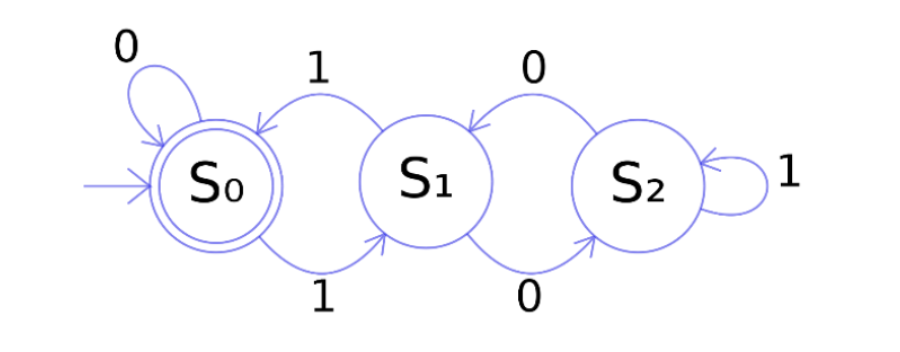
\includegraphics[width=16cm]{state_machine.png}}
\end{center}

\hfill \break
Depending on the current state and the input bit, the state machine transits from one state to another, as shown in the following diagram. The numbers in the state names (S0, S1, and S2) are the remainder when we divide by 3 the bits that the machine has seen. If the state is S0, the bits are divisible by 3.

\hfill \break
Implement the state machine in MyHDL. The skeleton code is in q2.py. We can complete the design in 3 steps. Steps 2 and 3 are the combinational circuit.

\begin{itemize}
    \item \textbf{Step 1} Instantiate a register to keep the state. We leverage the Register block that is provided in the skeleton code. The input and output signals of the state register have already been created.
    \item \textbf{Step 2} Complete the $next\_state\_logic()$ function, which generates the state to be saved in the state register in the next cycle.
    \item \textbf{Step 3} Complete the $z\_logic()$ function, which generates the output signal z, which indicates whether the number is divisible by 3. The z signal only depends on the current state.
\end{itemize}

\break
\section{Deliverable}
\begin{lstlisting}[language=Python,frame=tb]
    @block 
    def Register(dout, din, clock, reset):
        @always_seq(clock.posedge, reset=reset)
        def seq_reg():
            dout.next = din

        return seq_reg

    @block
    def Detect3x(z, b, clock, reset):
        state = Signal(intbv(0)[2:])
        next_state = Signal(intbv(0)[2:])
        
        # Step 1 - Instantiating the register with the state and output
        reg = Register(state, next_state, clock, reset)

        @always_comb
        def next_state_logic():
            '''
            Step 2 - Generating the next clock cycle's state
                        based on the current state, and the input bit
            '''
            next_state.next = state[1] ^ state[0] ^ b

        @always_comb
        def z_logic():
            # Step 3 - Generating the output based on the current state
            z.next = 1 if state == 0 else 0

        return instances()
\end{lstlisting}

\section{Results}
Below is the output of the state machine given eight randomly selected bits as input - 11101001.

\begin{table}[h]
    \centering
    \caption{State Machine Output}
    \begin{tabular}{|l|
        >{\columncolor{green!20}}l |
        >{\columncolor{green!20}}l |}
        \hline
        \textbf{b} & \textbf{z} & \textbf{v} \\ \hline
        1 & 0 & 1 \\ \hline
        1 & 1 & 3 \\ \hline
        1 & 0 & 7 \\ \hline
        0 & 0 & 14 \\ \hline
        1 & 1 & 29 \\ \hline
        0 & 1 & 58 \\ \hline
        0 & 1 & 116 \\ \hline
        1 & 0 & 233 \\ \hline
    \end{tabular}
\end{table}

\break
\section{Question 5}
Translate the following C function to RISC-V assembly code. The function converts an unsigned number into a string that represents the number in decimal. For example, after the following function call, the string placed in buffer is “3666”.

\begin{lstlisting}[language=C]
    uint2decstr(buffer, 3666);
\end{lstlisting}

\hfill \break
Assume the caller has allocated enough space for the string. Skeleton code is in q5.s, where the function is empty. Clearly mark in comments how each statement is translated into instructions.

\hfill \break
\begin{lstlisting}[language=C]
    char* uint2decstr(char* s, unsigned int v)
    {
        unsigned int r;
        if (v >= 10) {
            s = uint2decstr(s, v / 10);
        }
        
        r = v % 10; // remainder
        s[0] = "0" + r;
        s[1] = 0;
        return &s[1]; // return the address of s[1]
    }
\end{lstlisting}

\section{Deliverable}
\begin{lstlisting}[language=Assembler]
    uint2decstr:
        addi  sp, sp, -16               # allocate 16 bytes on the stack
        sw    ra, 12(sp)                # preserve ra by putting it on the stack
        sw    s0, 8(sp)                 # load s0 with the address of the string
        mv    s0, a1                    # load s0 with the value of v
        addi  a5, x0, 10                # load a5 with the value of 9
        bgeu  a1, a5, recurse           # if v > 10, call recurse

    write:
        addi  a1, x0, 10                # load a1 with the value of 10
        remu  s0, s0, a1                # s0 = v % 10
        addi  s0, s0, 48                # s0 = s0 + 48
        sb    s0, 0(a0)                 # store the result in the string
        sb    x0, 1(a0)                 # store the null terminator
        addi  a0, a0, 1                 # increment the address of the string
        lw    ra, 12(sp)                # restore ra
        lw    s0, 8(sp)                 # restore s0
        addi  sp, sp, 16                # move stack pointer back
        jr    ra                        # return to caller

    recurse:
        addi  a1, x0, 10                # load a1 with the value of 10
        divu  a1, s0, a1                # a1 = v / 10
        auipc t0, 0                     # save current address in t0
        jalr  ra, t0, 0xFFFFFFB8 # invoke write
        jal   write
\end{lstlisting}

\end{document}
